\chapter*{Criação de um projeto Dynamic Web Project no Eclipse Luna}
\label{apendice:1}
\captionsetup[figure]{list=no}
	
	\par Para proceder com a criação de um projeto do tipo \textit{Dynamic Web
Project} no Eclipse, é necessário acessar na IDE, a opção \textbf{File -> New->
Dynamic Web Project} como pode ser visto na Figura \ref{fig:desws3}.

	
	\begin{figure}[h!]
		\centerline{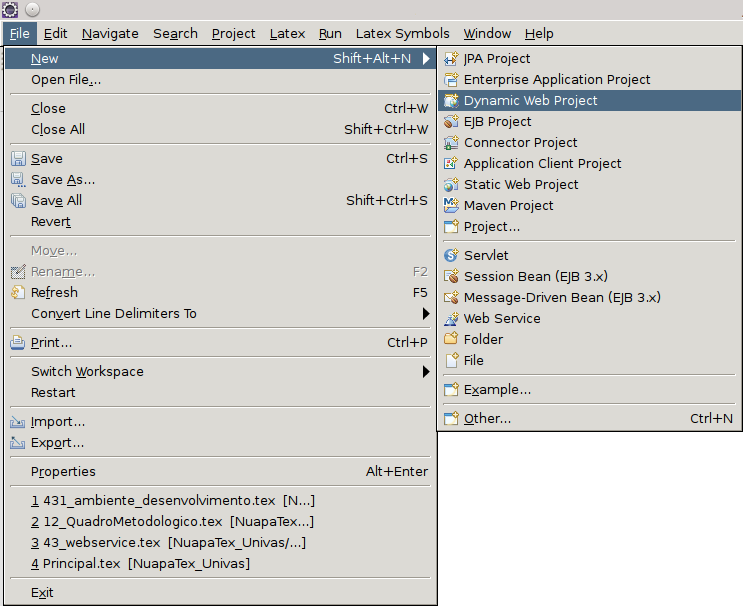
\includegraphics[scale=0.8]{./imagens/2_q_metodologico/4_procedimentos_resultados/43_webservice/432_desenvolvimento/desws3.png}}
		\caption[Tela \textit{New Database\ldots}]{Tela \textit{New Database\ldots}.
			\textbf{Fonte:}Elaborado pelos autores.}
		\label{fig:desws3}
	\end{figure}
	
	\pagebreak
	
 	\par Em seguida foi apresentada uma tela para o preenchimento de alguns dados
 requeridos para a criação do projeto. Destas informações somente foi preenchido
 o nome do projeto. As outras informações continuaram sendo as que vem por
 padrão da IDE. A janela apresentada e as informações preenchidas podem ser
 vistas na Figura \ref{fig:desws4}.

	\begin{figure}[h!]
		\centerline{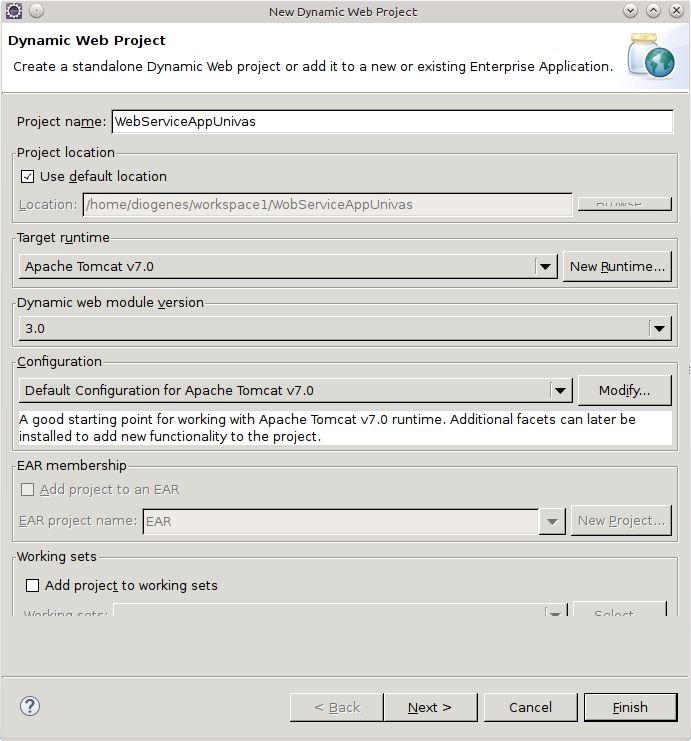
\includegraphics[scale=0.8]{./imagens/2_q_metodologico/4_procedimentos_resultados/43_webservice/432_desenvolvimento/desws4.png}}
		\caption[Tela para criação de um novo projeto no Eclipse]{Tela para criação de um novo projeto no Eclipse.
			\textbf{Fonte:}Elaborado pelos autores.}
		\label{fig:desws4}
	\end{figure}
	
	\pagebreak
	
	
	\par Na próxima janela apresentada, que têm por função configurar a pasta de
códigos do projeto manteve-se a configuração apresentada pela IDE, como mostra
a Figura \ref{fig:desws5}.

	\begin{figure}[h!]
		\centerline{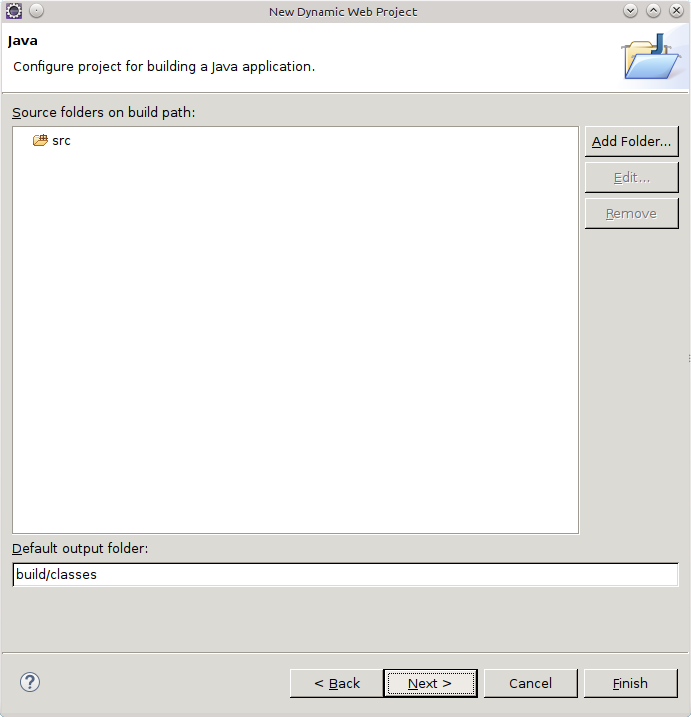
\includegraphics[scale=0.8]{./imagens/2_q_metodologico/4_procedimentos_resultados/43_webservice/432_desenvolvimento/desws5.png}}
		\caption[Tela para criação de um novo projeto no Eclipse]{Tela para criação de um novo projeto no Eclipse.
			\textbf{Fonte:}Elaborado pelos autores.}
		\label{fig:desws5}
	\end{figure}
	
	\pagebreak
	
	\par Na sequência, na tela que foi apresentada era necessário preencher o
campo \textbf{Context root} com o contexto principal da aplicação web que
acabou mantendo o próprio nome da aplicação. Além disso foi marcado a opção
\textbf{Generate web.xml deployment descriptor}, para que ao criar o projeto, a
própria IDE criasse o arquivo \texttt{web.xml}, arquivo responsável por algumas
configurações da aplicação web. Esta tela está apresentada na Figura
\ref{fig:desws6}.

	\begin{figure}[h!]
		\centerline{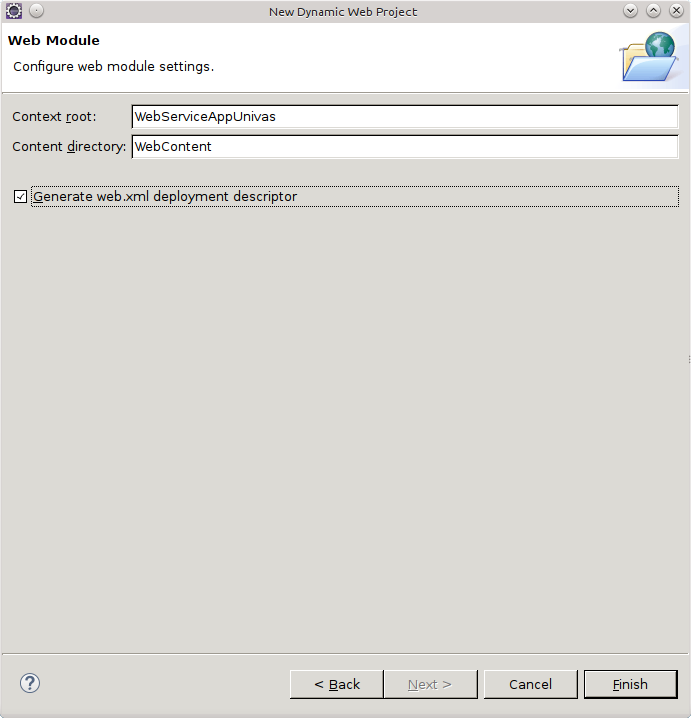
\includegraphics[scale=0.8]{./imagens/2_q_metodologico/4_procedimentos_resultados/43_webservice/432_desenvolvimento/desws6.png}}
		\caption[Tela para criação de um novo projeto no Eclipse]{Tela para criação de um novo projeto no Eclipse.
			\textbf{Fonte:}Elaborado pelos autores.}
		\label{fig:desws6}
	\end{figure}
	
	\pagebreak

	%03 - Mapeamento orm;	
		%	->Criação do pacote

	\par Após este passo foi concluído a criação do projeto.
	%, e já era possível iniciar os trabalhos com a camada de persistência de dados
	% do projeto.
